\section{Analysis of the Okazaki Fragment Distributions along Single Long DNAs}

\subsection{Нормальное название}

Исследование распределения фрагментов Окадзаки вдоль одиночных длинных ДНК, реплицируемых белками бактериофага T4.  

\subsection{Абстракт}

Репликация типа катящегося кольца в кольцах ДНК бактериофага М13 была ранее воссозданна инвитро, используя очищенные факторы, кодируемые бактериофагом Т4. Её продуктами являются двунитевые кольца с линейными хвостами >100 kb. При использовании ДНК-полимеразы бактериофага Т4, дефицитной по экзонуклеазной активности от 3 ’до 5’, электронная микроскопия выявила короткие «лоскуты» одноцепочечной ДНК вдоль реплицированных хвостов. Последнии определяли начало каждого фрагмента Окадзаки, что позволило проанализировать длину последовательных фрагментов Окадзаки на отдельных реплицирующихся молекулах. Были обнаружены ДНК, содержащие серии фрагментов Окадзаки одинаковой длины, однако большинство из них демонстрировали большое разнообразие длин в сериях из шести или более фрагментов, что отражает широкое распределение популяции.

\subsection{Картинки}


\paragraph{Рисунок 1}


\begin{figure}[h]
\begin{minipage}[h]{0.49\linewidth}
\center{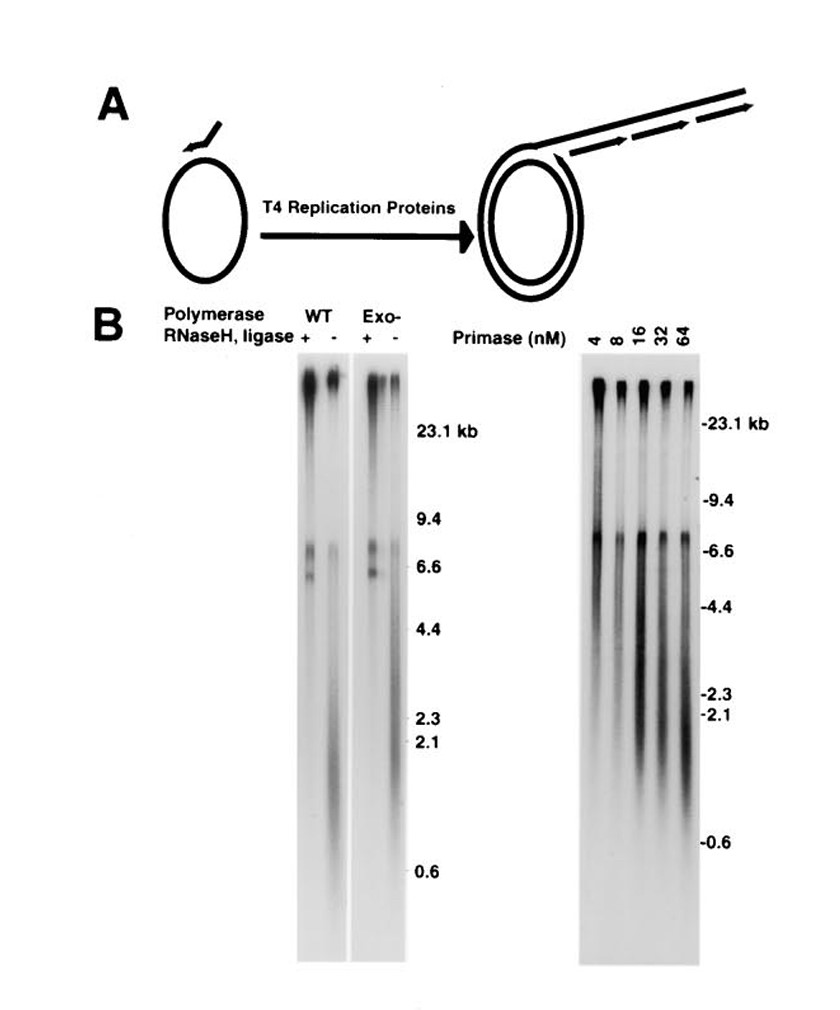
\includegraphics[width=\linewidth]{5_1} }
\end{minipage}
\hfill
\begin{minipage}[h]{0.49\linewidth}
\center{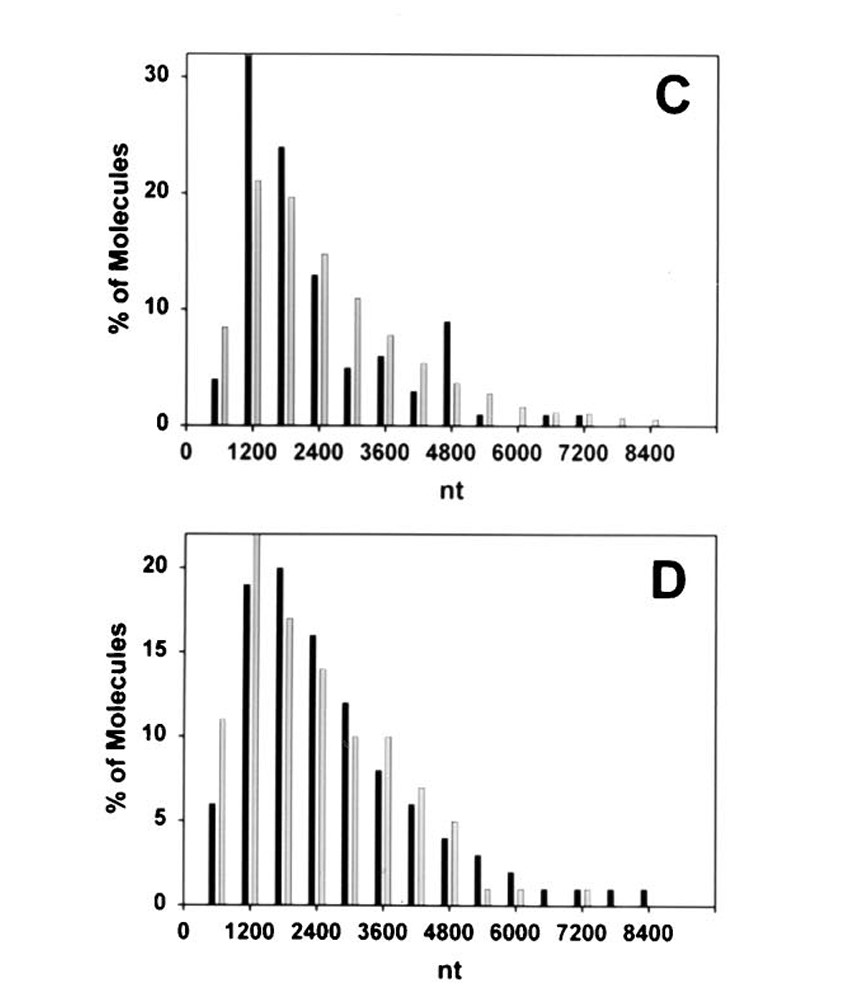
\includegraphics[width=\linewidth]{5_2} }
\end{minipage}
\label{fig:5_12}
\caption{Рисунок 1}
\end{figure}


A: Фото показывает, как происходит репликация по типу катящегося кольца. Фрагменты Оказаки показаны на правой картинки с помощью стрелочек. Полимераза показана на левой картинке маленьким хвостиком над кольцом.
B: Результаты электрофореза. Если есть рнказа и лигаза( там плюс есть) видим четкие полоски около 6000 нуклеотидов( 6 kb). Это соответствует полному кольцу двунитевой днк. Совсем сверху( выше 23 kb) – вариант, когда длинный-длинный хвост двунитевой получился. Это наблюдается независимо от того есть экзонуклеазная активность у полимеразы или ее нет. Если нет рнказы и лигазы, то видим, что нет полного кольца, очень мало большого продукта сверху на рисунке, и широкое пятно около 2 kb. Это фрагменты Оказаки, потому что нет рнказы и лигазы, все фрагменты Оказаки находятся отдельно друг от друга, несшиты друг с другом и в таком случае будут двигаться по отдельности широким фронтом. Дальше на правой картинке меняют концентрацию праймазы. Чем больше праймазы дадим, тем чаще будет образовываться праймер на реплицированной нити, тем короче будут фрагменты Оказаки. От концентрации праймазы зависит длина фрагмента Оказаки.

C и D: В (С) реакция катализировалась мутантной ДНК-полимеразой D219A в отсутствие РНКазы Н и ДНК-лигазы, а в (D) реакция катализировалась ДНК-полимеразой дикого типа с РНКазой Н и ДНК-лигазой. В отсутствие РНКазы Н и лигазы (С) сравниваются все фрагменты Окадзаки, в то время как в (D) сравниваются только самые последние синтезированные фрагменты.

\paragraph{Рисунок 2}

\begin{figure}[h]
\begin{minipage}[h]{0.49\linewidth}
\center{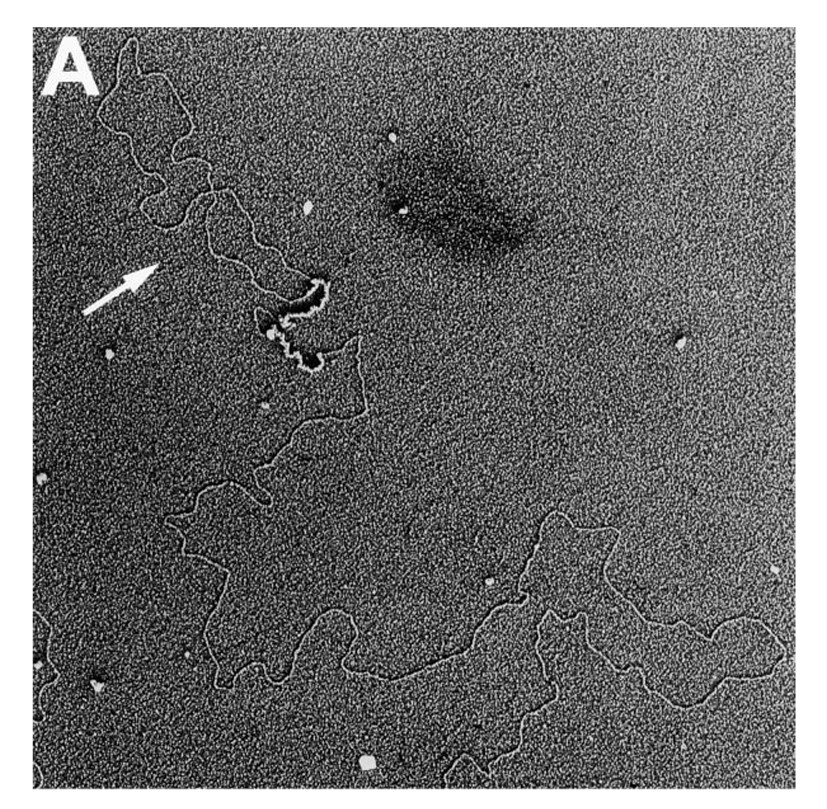
\includegraphics[width=\linewidth]{5_3} }
\end{minipage}
\hfill
\begin{minipage}[h]{0.49\linewidth}
\center{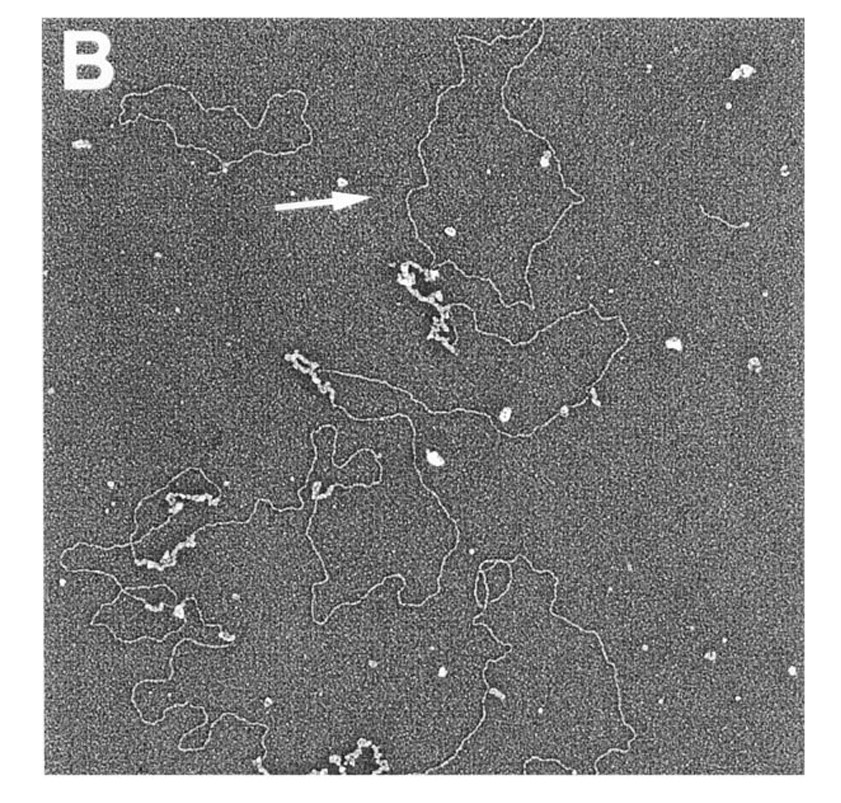
\includegraphics[width=\linewidth]{5_4} }
\end{minipage}
\caption{Рисунок 2}
\label{fig:5_34}
\end{figure}

Визуализация продуктов репликации, катализируемых ДНК - полимеразой Т4 дикого типа. На рисунке А показана репликация проводилась с использованием рнказой и лигазой, а на рисунке В – без них. Стрелочки показывают на кольца днк. Утолщения на картинке А – это белки ssB( белки, которые связываются с однонитевой днк). Они добавлены, чтобы визуализировать однонитевые участки. На рисунке В, когда нет рнказы и лигазы, появляются однонитевые участки на границе между двумя фрагментами Оказаки, потому что полимераза не может сшить два фрагмента и случайным образом оказывается, появляется пробел между этими фрагментами, которые благодаря белкам можем наблюдать( толстые белые участки).\

\paragraph{Рисунок 3}

Визуализация продуктов репликации, катализируемых ДНК-полимеразой D219A T4( мутантный тип). Суть такой полимеразы в том, что она отсоединяет хвост ранее синтезированного фрагмента Оказаки от матрицы.

Реакции репликации типа катящегося колеса проводили, как описано на фиг. 1 и 2, с использованием ДНК-полимеразы D219A T4 без РНКазы H и ДНК-лигазы.  После инкубации в течение 5 мин образцы депротеинизировали и готовили для ЭМ (электромикроскопии), как описано на фиг. 2. Стрелки указывают кружки-матрицы M13 (“колёса”).  Из-за свойств инвазии цепи мутантной полимеразы D219A предполагалось, что на стыке каждого завершенного фрагмента Окадзаки (вставка) будут образовываться лоскуты оцДНК.  Примаза присутствовала в количестве 64 нМ (A и B) или 8 нМ (C).  На фото A насчитывается 23 фрагмента Окадзаки , 4 на B и 6 на C. Лоскуты, окрашенные SSB, имеют тенденцию быть длиннее с при пониженном количестве примазы (C).  Изображения сделаны с обратным контрастом: столбик соответствует длине дцДНК, эквивалентной 1,1 т.п.н. (A), 1,0 т.п.н. (B) или 0,8 т.п.н. (C).

\begin{figure}[h]
    \centering
    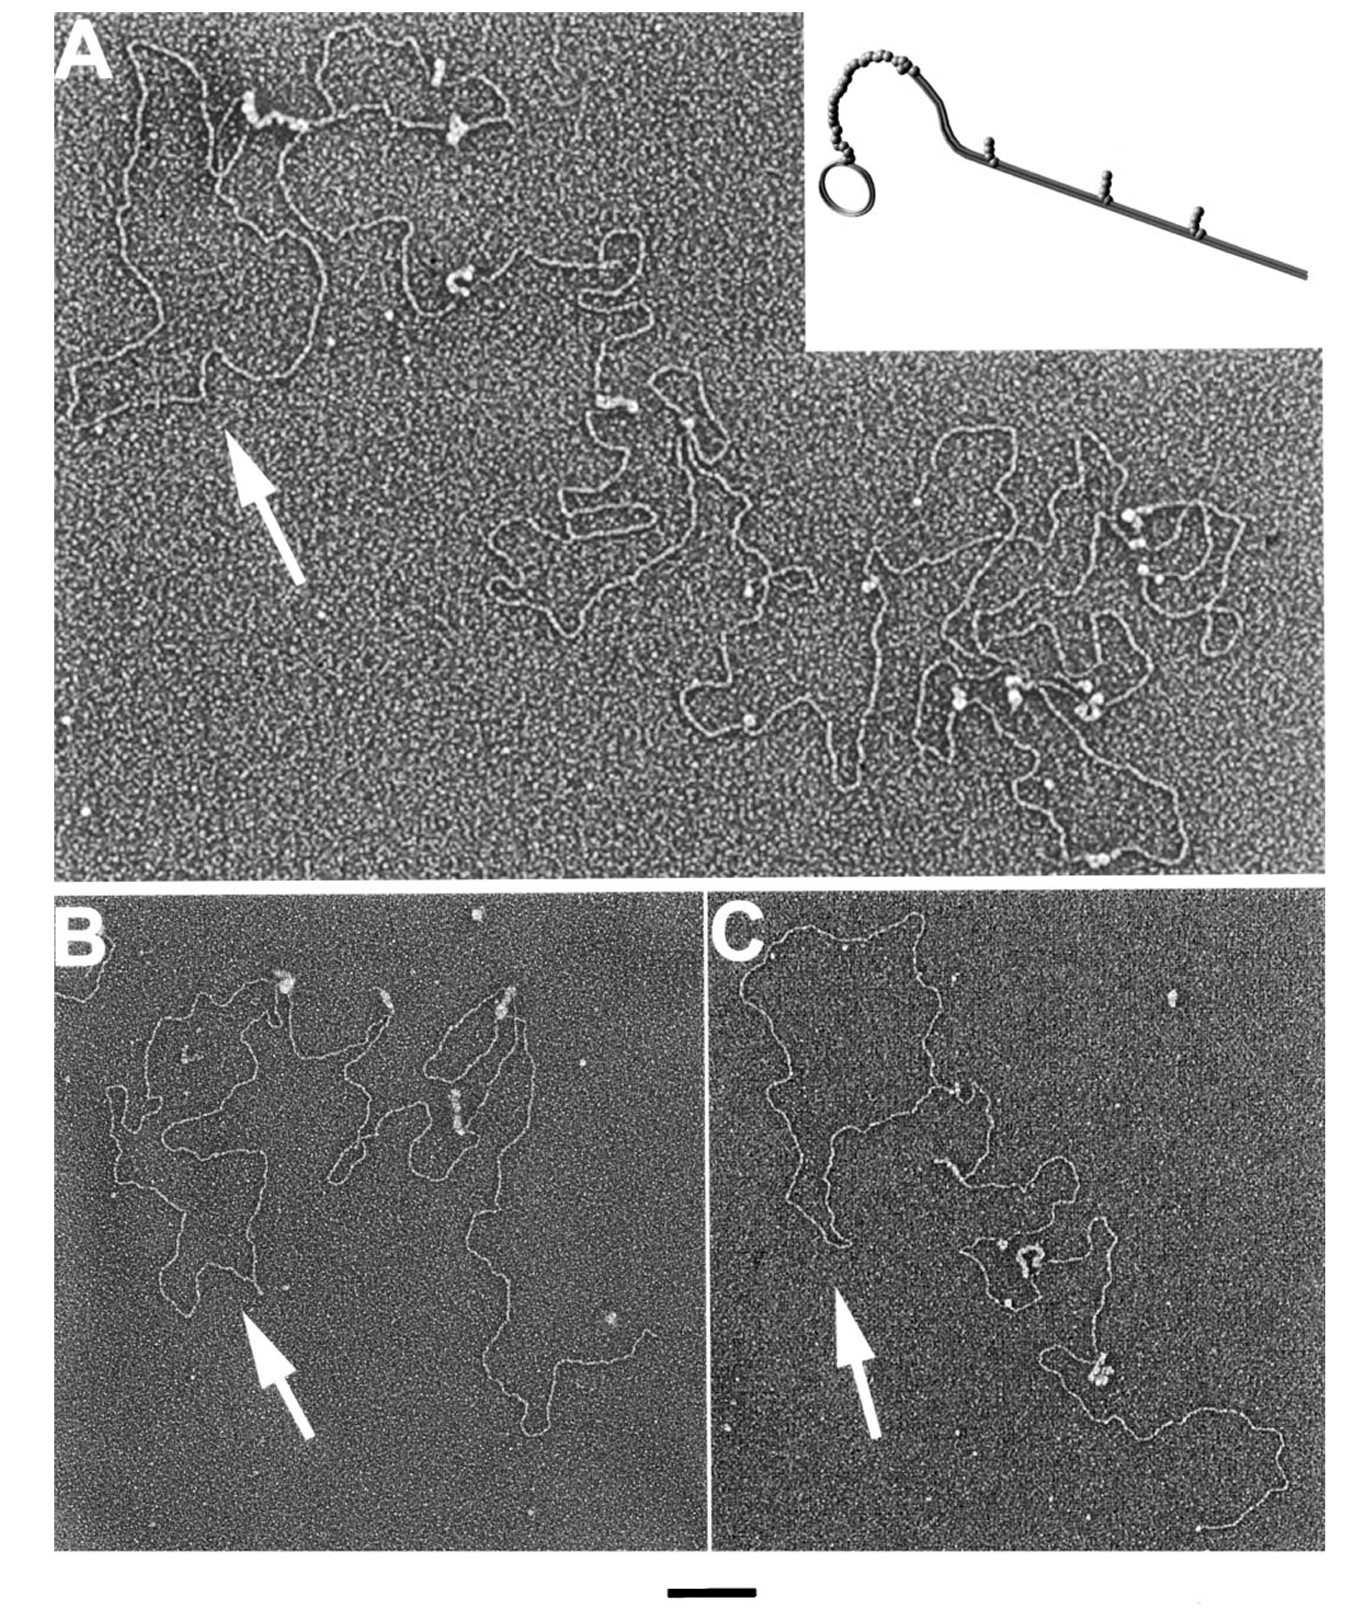
\includegraphics[width=0.5\linewidth]{5_5}
    \caption{Рисунок 3}
    \label{fig:5_5}
\end{figure}

\paragraph{Рисунок 4}

Определение длины фрагментов Окадзаки с помощью ЭМ (электромикроскопических снимков).

(A)	Фрагмент Окадзаки в процессе синтеза состоит из двух сегментов, дуплексной области (ds1) и одноцепочечной области (ss2).  Первый соответствует количеству произошедшего синтеза отстающей цепи, а второй соответствует оставшейся синтезируемой матрице.
(B)	Завершенный фрагмент Окадзаки, продуцируемый мутантной полимеразой D219A в отсутствие РНКазы H и лигазы, состоит из трех сегментов, смещенной области (flap1), дуплексной области (ds1) и лоскута, образованного вторжением в следующий фрагмент (flap2).  Flap 1 соответствует количеству ДНК  вымещенному мутантов полимеращой D219A преобразовании следующего отрезка Окадзаки.  Сегмент ds1 соответствует дуплексной части измеряемого фрагмента Окадзаки.  Flap2 соответствует длине ДНК соседнего фрагмента Окадзаки, вытесненной мутантной полимеразой.

\begin{figure}[h]
    \centering
    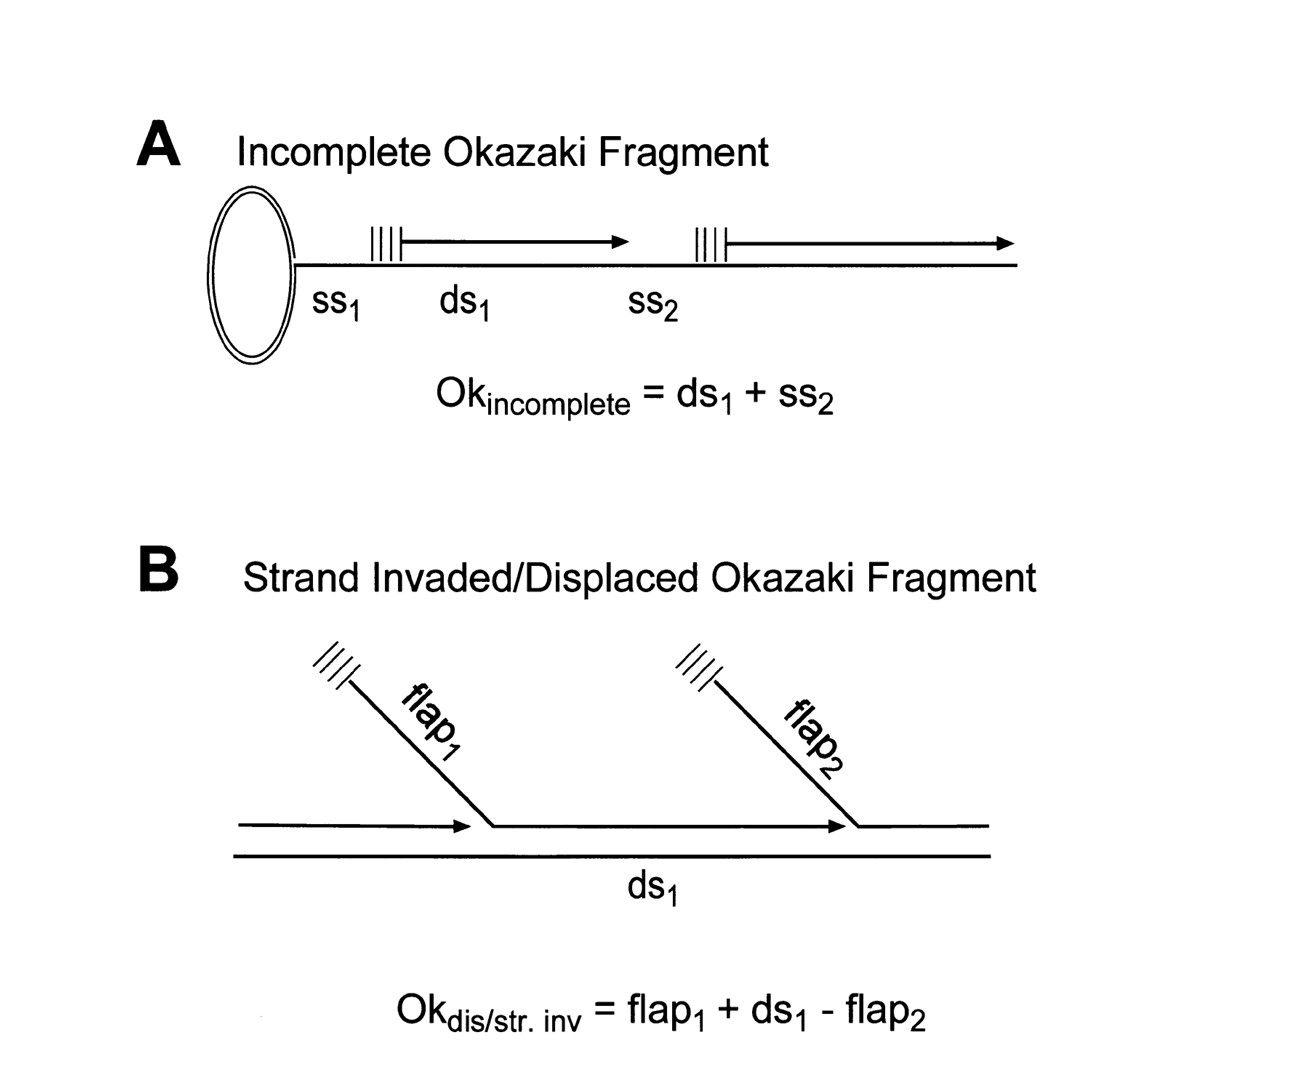
\includegraphics[width=0.5\linewidth]{5_6}
    \caption{Рисунок 4}
    \label{fig:5_6}
\end{figure}

\paragraph{Рисунок 5}

Распределения последовательных фрагментов Окадзаки, являющихся продуктами длинной репликации типа катящегося колеса. 

Из микрофотографий, таких как те, что на рисунке \ref{fig:5_5}, и критериев измерения, описанных на рисунке \ref{fig:5_6}, была определена длина последовательных фрагментов Окадзаки, расположенных вдоль хвостов круговой матрицы, генерируемых ДНК-полимеразой D219A в отсутствие РНКазы H и лигазы.  Длина каждого фрагмента показана по оси y, а суммарное расстояние от конца ДНК, удаленного от круглой матрицы, показано по оси x.  Ориентация показана на рисунке.  Примеры распределений фрагментов, синтезированных в присутствии 64 нМ (A – F) или 8 нМ (G – L) примазы.
\begin{figure}[H]
\centering
    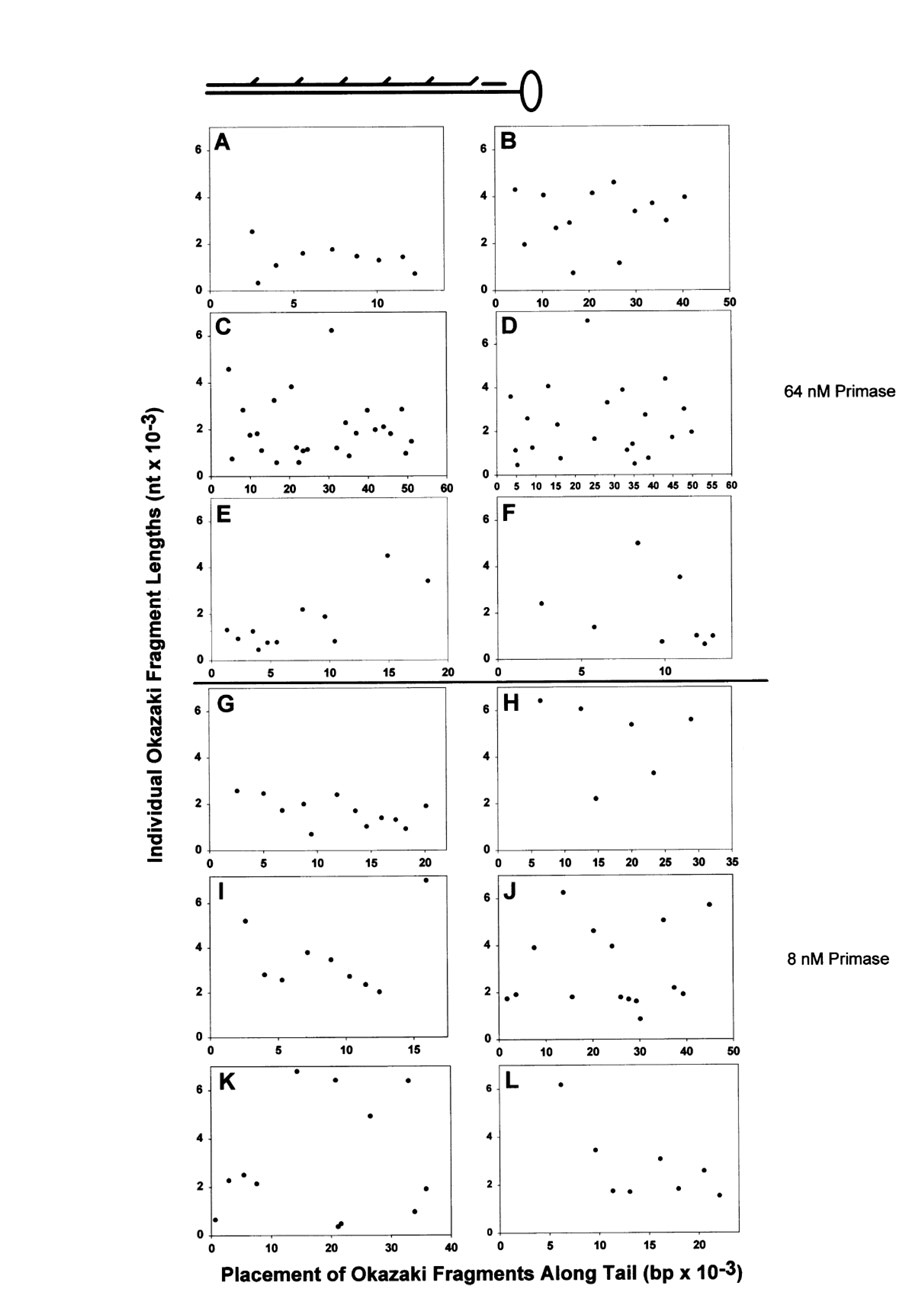
\includegraphics[width=0.5\linewidth]{5_7}
    \caption{Рисунок 5}
    \label{fig:5_7}
\end{figure}

\paragraph{Рисунок 6} Сравнение распределений фрагментов Оказаки для одной реплицирующейся молекулы с общей популяцией. 

Длины фрагментов Окадзаки вдоль отдельных реплицирующихся молекул, взятые из таблиц 1 и 2 (A и B, соответственно), были нанесены на сглаженные логарифмически нормальные распределения (тонкие линии; значения оси Y слева) и сравниваются с общей популяцией фрагментов Окадзаки.  длины построены аналогично (жирная линия; значения оси Y справа).  Реакции происходят с примазой 64 нМ (A) и 8 нМ (B).

\begin{figure}[H]
\begin{minipage}[h]{0.49\linewidth}
\center{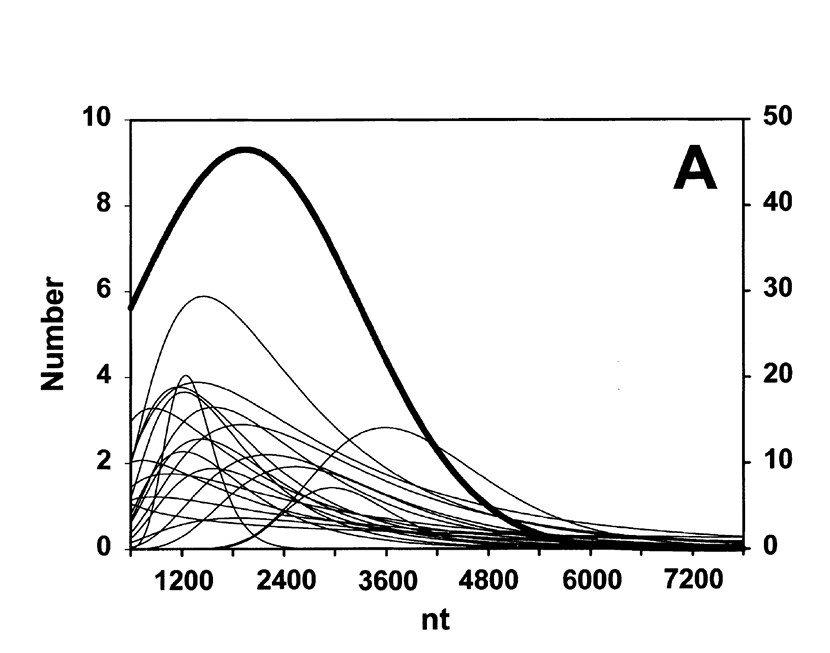
\includegraphics[width=0.8\linewidth]{5_8} }
\end{minipage}
\hfill
\begin{minipage}[h]{0.49\linewidth}
\center{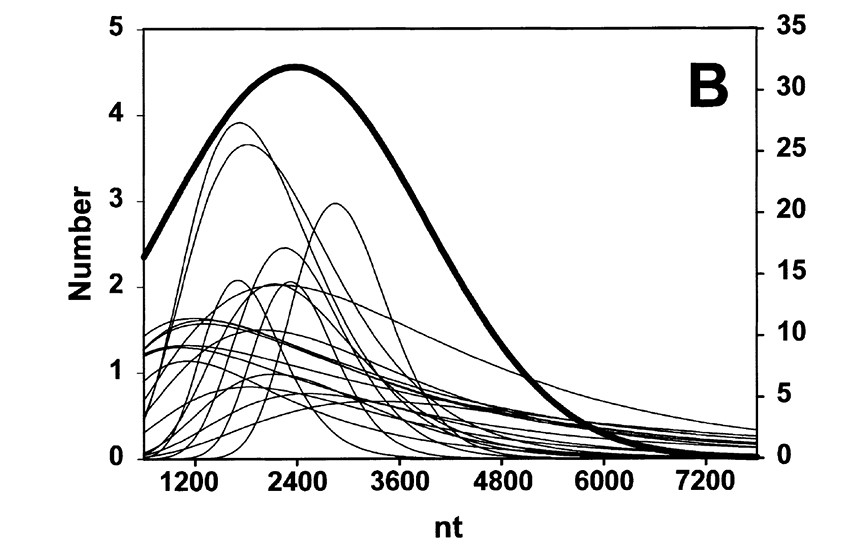
\includegraphics[width=0.8\linewidth]{5_9} }
\end{minipage}
\caption{Рисунок 6}
\label{fig:5_89}
\end{figure}

\newpage